\subsection{Word segmentation}
\label{sec:segmentation}

%    we used the same datasets for the full classifier and the one based on single units. In both cases, we could train them on 100 and 10k examples, for consistency? Or maybe just use 10k in all cases, explaining in the text why we use this size, and maybe even remarking that performance is well above chance also with much less data?

We tested whether our CNLM developed an implicit notion of word, despite not being endowed with a hard-coded word dictionary, and being exposed to unsegmented input. %
To answer this, we return to the method of diagnostic classifiers.
We randomly selected positions from the development partition such that half of these were the last character of a token, and the other half were not.
We collected 10000 such points as training data for the diagnostic classifiers, and the remainder for testing.
Both sets were balanced between (1) and (2).
We sampled the test data points subject to the constraint that the word or word prefix ending at the selected character does not overlap with the training set.
This ensures that the diagnostic classifier cannot succeed by looking for encodings reflecting specific words.



We compared this to the following lexicon-based classifier:
Given a position where the last word is $x_1...x_n$, we count how often $x_1...x_n$ occurs as a token in the tokenized Wikipedia training set ($N_1$), and how often a longer word starting with $x_1...x_n$ occurs there ($N_2$).
The classifier guesses that a boundary is present if $N_1 > N_2$, and that no boundary is present if $N_1 < N_2$, and guesses randomly if $N_1 = N_2$.
This is a very strong classifier:
First, unlike the CNLM, it has oracle access to the beginning of the current word.
With this, it represents the \emph{optimal} classifier for this task when the beginning of the current word is known, but the prior context is not given.
Furthermore, it has access to a very large lexicon listing all unigram counts in the training corpus, encoding a vast amount of lexical knowledge and proper names.

Results are shown in Table~\ref{tab:segmentation-results}.
We find that the diagnostic classifier shows above-random performance with few training samples, though its performance lags behind that of the single-parameter classifiers derived from the units we found above, suggesting overfitting of the diagnostic logistic classifier.
With 1000 training samples, the diagnostic classifier performs similarly to the strong lexicon-based classifier, and outperforms it with 10,000 training samples.
This shows that the CNLM's representations provide strong cues regarding word boundaries.
Performance is strongest in English and weakest in German, both for the CNLM-based diagnostic classifier and for the lexicon-based baseline.
The preponderance of compound words in German may be responsible for this.




\begin{table}[t]
	\small
  \begin{center}
    \begin{tabular}{l|l|l|l}
      \multicolumn{1}{c|}{}&\emph{LSTM}&\emph{RNN}&\emph{Lexicon}\\
      \hline
      English & 72.7/89.9/91.8 &  66.6/76.8/84.5  &  88.7   \\ 
      German & 61.8/79.8/87.6  &  61.5/75.8/84.3 &  79.3  \\ 
      Italian &  60.7/83.0/90.2 &  69.1/75.9/86.6  &  84.2   \\ 
    \end{tabular}
  \end{center}
  \caption{\label{tab:segmentation-results} Accuracy of diagnostic classifier on recognizing word boundaries, with 100/1000/10000 training samples. Random baseline accuracy is 50 \%.}
\end{table}



\newcite{Kementchedjhieva:Lopez:2018} found a unit that tracks morpheme boundaries, using an English CNLM that was trained with whitespace (unlike our CNLMs).
We applied the following method to probe whether our CNLMs had developed such units, even in the absence of any whitespace in the input.
For each language, we randomly chose 10,000 positions from the training set, balanced between positions that were the last character of a word, and word-initial/word-medial positions.
We then computed, for each hidden unit of the CNLMs, the Pearson correlation between its activations and the indicator that is 1 for word-final positions and 0 otherwise.
For each language and model (LSTM and RNN), we selected the unit with the highest correlation.
For the LSTM CNLMs, we found correlations of 0.58 (English), 0.69 (German), 0.57 (Italian).
For the RNN CNLMs, the highest correlations were 0.40 (English), 0.46 (German), 0.46 (Italian).
%Note that the models can have further 
%For LSTM CNLMs, we found at least 5 units with strong correlations ($>0.5$). For the RNN CNLMs, we also found at least one unit with correlation $> 0.4$ in each of the languages.

We then used the development partition to further investigate, for each language, the behavior of the unit that showed the strongest correlation.
The behavior of these units on sample sequences from the development partition is illustrated in Figure~\ref{fig:word-unit}.
Qualitatively, the unit consistently shows high activation on token boundaries, but also some peaks at word-medial positions.
In the German snippet, we see peaks at the morpheme boundaries of the compound \emph{Haupt-auf-gabe}.
To investigate how consistently this unit detects word boundaries, we trained a threshold classifier on this single unit (i.e., a classifier with a single parameter) on 1,000 positions from the development set, using the remainder as test data, predicting whether the last character read by the CNLM represents the end of a word, as tokenzied by TreeTagger.
For both the training and test data, we balanced the number of word-final and word-initial/word-medial positions.

We carried out the same procedure for the CNLMs we trained with whitespace, similar to the setup of \newcite{Kementchedjhieva:Lopez:2018}.
We expect that the explicit encoding of words would lead to even stronger encodings in such a network than in our CNLMs.

Test accuracies are shown in Table~\ref{tab:segmentation-unit-results}.
In all languages, the unit is strongly predictive of word boundaries, clearly outperforming the random baseline of 50 \% in our balanced test set.
Across languages, the LSTM CNLM units are more predictive than the RNN ones, and, across the three languages, competitive with those derived from a CNLM that was trained with whitespace.


% English /home/user/CS_SCR/FAIR18/CHECKPOINTS/boundary-neuron//
% Italian /home/user/CS_SCR/FAIR18/CHECKPOINTS/boundary-neuron//
% German /home/user/CS_SCR/FAIR18/CHECKPOINTS/boundary-neuron//

\begin{figure*}
	\includegraphics[width=0.9\textwidth]{figures/{english_wiki-english-nospaces-bptt-282506230_15.txt}.png}
	\includegraphics[width=0.9\textwidth]{figures/{german_wiki-german-nospaces-bptt-910515909_12.txt}.png}
	\includegraphics[width=0.9\textwidth]{figures/{italian_wiki-italian-nospaces-bptt-855947412_7.txt}.png}
	\caption{Behavior of the CNLM `word unit' in English, German, and Italian, with word boundaries marked in green. TODO do we need to find a better Italian example?}\label{fig:word-unit}
\end{figure*}

\begin{table}[t]
	\small
  \begin{center}
    \begin{tabular}{l|l|l||l}
      \multicolumn{1}{c|}{}&\emph{LSTM}&\emph{RNN}&\emph{LSTM} with whitespace\\
      \hline
	    English & 77.5 & 65.6 & 83.2 \\ 
	    German & 80.8 & 66.8  & 71.3  \\ 
	    Italian & 75.4 & 71.6 & 78.1 \\ 
    \end{tabular}
  \end{center}
  \caption{\label{tab:segmentation-unit-results} Accuracy of threshold classifier based on `word' unit in distinguishing word boundaries from word-internal positions. Random baseline accuracy is 50 \%.}
\end{table}

To better understand the behaviour of the LSTM CNLM word unit, we
conducted a qualitative analysis of cases where it under- or
oversegments orthographic words. We discuss German here, as it is the
language where the word-unit classifier reaches highest accuracy, and
its tendency to have long, morphologically complex words makeis
particularly interesting. However, similar patterns were also detected
in Italian and, to a lesser extent, English (in the latter, there are
fewer and less interpretable common oversegmentation, probably because
words are on average shorter and morphology more limited). Considering
first the 30 most common undersegmentations of the word-unit
classifier, the large majority (24/30) are common sequences of
grammatical terms or very frequent items that can sometimes be
reasonably be re-analyzed as single function words or adverbs (e.g.,
\emph{bis zu}, `up to (lit.~until to)', \emph{je nach} `depending on
(lit.~per??? after)', \emph{bis heute} `to date (lit.~until
today)'). 3 cases are multi-word city names (\emph{Los Angeles}). The
final 3 cases interestingly involve \emph{Bau} `building' followed by
\emph{von} `of' and genitive determiners \emph{der/des}. As in its
eventive reading this noun requires a patient licensed by either `of'
or (in German) genitive (\emph{Bau der Mauer} `building of the wall
(lit.~ building the-GEN wall)'), apparently our model decided to
absorb the case assigner into the form of the noun.

We looked next at the 30 most common oversegmentations of the
word-unit classifier (defines as the character substrings that were
wrongly segmented out of the largest number of distinct words),
limiting the analysis to those containing at least 3 characters, as
shorter strings were more ambiguous and harder to interpret. Of these,
6 are prefixes that can also occur in isolation as prepositions or
verb particles (\emph{auf} `on', \emph{nach} `after', etc.). 7 are
content words that form many compounds (e.g., \emph{haupt} `main',
occurring in \emph{Hauptstadt} `capital', \emph{Hauptbahnhof} `main
station' etc.; \emph{Land} `land', occurring in \emph{Deutschland}
`Germany', \emph{Landkreis} `district', etc.). Another 7 items can be
classified as suffixes (e.g., \emph{-lich} as in \emph{s\"udlich}
`southern', \emph{wissenschaftlich} `scientific'), although their
segmentation is not always canonical (e.g., \emph{chaft} instead of
the expected \emph{schaft} in \emph{Wissenschaft} `science'). 4 very
common function words are often wrongly segmented out of longer words
(e.g., \emph{sie} `she' from \emph{sieben} `seven'). The \emph{kom}
and \emph{kon} cases are interesting, as the model seems to both
correctly segment these as reasonable stem forms of the verbs
\emph{kommen} `to come' and \emph{kennen} `to know', respectively
(e.g., in \emph{kommt} and \emph{konnte}, respectively), and as
pseudo-prefixes elsewhere (\emph{komponist} `composer', \emph{kontakt}
`contact'). The remaining 3 oversegmentations, \emph{rie}, \emph{run}
and \emph{ter} don't have any clear interpretation.

Taken together, the error analysis highlights the fact that the
``word'' unit, even when analyzed through the lens of a threshold that
was optimized on word-level segmentation, is actually tracking
``salient'' linguistic boundaries at different levels. While in many
cases these boundaries naturally coincide with words (hence the high
quantitative performance of the simple classifier), the CNLM is also
sensitive to frequent morphemes and compound elements, as well as to
different types of multi-word expressions. This is fully in line with
a view of wordhood as a useful but ``soft'', emergent property, rather
than with the traditional assumption of words as rigid primitives of
linguistic processing.





% python detectBoundariesUnit_Hidden_ExtractPattern_NoWhitespace_Classifier.py --language english  --batchSize 128 --char_dropout_prob 0.001 --char_embedding_size 200 --char_noise_prob 0.0 --hidden_dim 1024 --language english --layer_num 3 --learning_rate 3.6  --myID 282506230 --load-from wiki-english-nospaces-bptt-282506230 --weight_dropout_hidden 0.01 --weight_dropout_in 0.0
% output in 
% results/segmentation-english-frequent-errors-unit-disjoint.txt





%
%
%
%
%
%\textbf{TODO} I think we may not need the syntactic depth experiment, as the PMI measure is not used anywhere else.
%
%We have found that the hidden state of the CNLM encodes information about word boundaries.
%We now investigate whether the probabilities computed by the CNLM are reflective of boundaries.
%We considered the pointwise mutual
%information (PMI) between left and right contexts, computed by
%subtracting the unconditional log-likelihood of the next 20 characters
%from their log-likelihood conditioned on the prior context.
%We created constituency trees for the German
%validation set using the Berkeley Parser~\cite{petrov2007improved}, using the provided German model\footnote{https://github.com/slavpetrov/berkeleyparser}.
%For each character in the data, we counted its hierarchical distance
%from the preceding character, operationalized as the number of
%intervening closing and opening brackets.  This number is zero if both characters belong to the same word, 1 at word
%boundaries, larger at larger-constituent boundaries. Figure~\ref{fig:syntax-depth} plots CNLM-based PMI by
%hierarchical distance, for all distances for which at least 1,000
%data-points occurred in the data-set.  The plot shows that longer
%hierarchical distance between neighboring characters correspond to
%lower average PMI.
%
%%This
%%illustrates how it is useful for segmentation knowledge to be
%%implicit, as the model can discover information about different kinds of
%%boundaries in a continuous manner.
%
%\begin{figure}
%  \center
%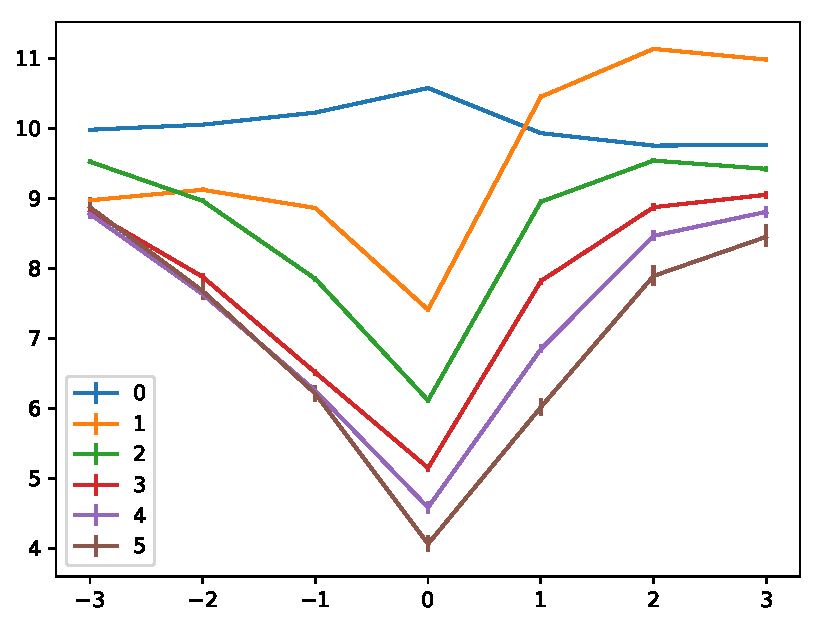
\includegraphics[width=0.4\textwidth]{figures/segmentation-profile-pmis-german-all-heights-ci.pdf}
%\caption{PMI between left and right contexts, as estimated by the LSTM CNLM in German, organized by syntactic hierarchical distance between subsequent characters (with bootstrapped 95 \% confidence intervals).}\label{fig:syntax-depth}
%\end{figure}
%
%
%
%%687112
%%73757
%%46716
%%22847
%7896
%2587
%827
%234
%80





%
%
%
%% (whitespace), if it is distilling meaningful linguistic knowledge, we
%% expect that it should develop some implicit notion of word-like units.
%Early work on word segmentation has shown that low transition
%probabilities \cite{harris-distributional-1954, saffran-word-1996},
%high uncertainty about the next character \cite{cohen-algorithm-2001,
%  feng-accessor-2004} and low mutual information
%\cite{sun-chinese-1998} serve as statistical cues to word
%segmentation.  %In Figure~\ref{fig:syntax-depth}, we plot (1) entropy
%% of the predicted distribution over the next character around word
%% boundaries, compared to other positions, and (2) the pointwise mutual
%% information (PMI) between left and right contexts, computed by
%% subtracting the unconditional log-likelihood of the next 20 characters
%% from their log-likelihood conditioned on the prior context, both computed
%% using our pre-trained LSTM on a section of the German training
%% set.  We see that higher entropy and lower PMI computed on
%% model-generated probabilities correlate with word boundaries,
%% suggesting that the model internalized statistics that cue segmentation.
%%
%% \begin{figure}
%% 	\begin{center}
%% 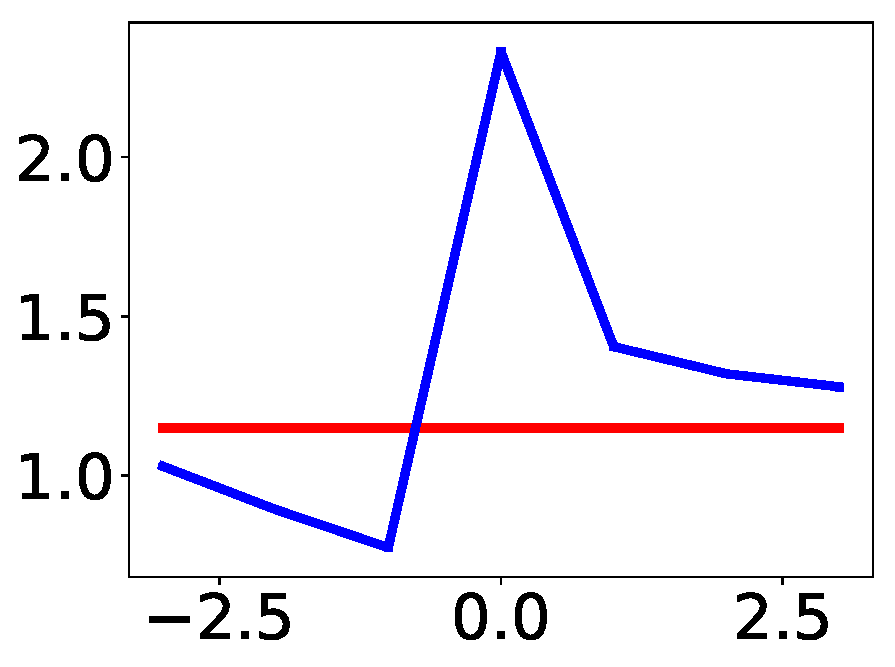
\includegraphics[width=0.22\textwidth]{figures/segmentation-profile-flattened-entropies-english-ci.pdf}
%% 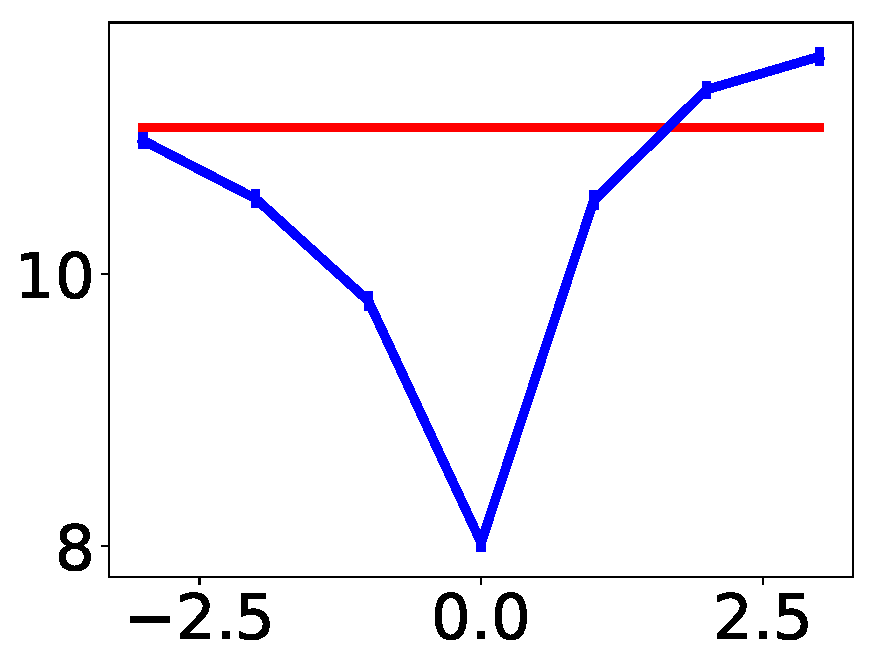
\includegraphics[width=0.22\textwidth]{figures/segmentation-profile-flattened-pmis-english-ci.pdf}
%% 	\end{center}
%% 	\caption{Average entropy over the next character (left) and PMI between left and right contexts (right) around word boundaries (blue); the x-axis indicates position relative to a word boundary. The red line indicates the overall average of the quantity. Error bars indicate (almost imperceptible) bootstrapped 95 \% confidence intervals.}\label{fig:boundaries-entropy}
%% \end{figure}
%%
%Based on these considerations, we tested the model segmentation
%capabilities as follows. We used the development sets to
%train  logistic classifiers predicting whether a character is first in
%a word or not, based on the following features, derived from the
%pre-trained CNLMs without further tuning: (1) \emph{surprisal}, the
%log-probability of the character given prior context, (2)
%\emph{entropy} of the distribution over the character given prior
%context, (3) \emph{context PMI}, that is, the total
% likelihood of the next 20 characters, minus the unconditional
% likelihood estimated by starting the CNLM at the current position. %
%%The rationale of (3) is that it measures the pointwise mutual information, and thus the statistical association, between the subsequent characters and the prior context, which we hypothesize will be higher inside words.
%%It is also the transition probability for the next characters
%%(3) can also be interpreted as the result of normalizi transition probability
% We collected these quantities for each position and the preceding
% and following three characters, resulting in a 21-feature classifier. %
%%In total, the classifier has 21 coefficients.
%We repeated the  experiment with features extracted from a
%character-level 8-gram model estimated on the training set, closer to
% earlier non-neural work
%\cite{saffran-word-1996, feng-accessor-2004}.
%
%
%\begin{table}[t]
%	\small
%  \begin{center}
%    \begin{tabular}{l|l|l|l}
%      \multicolumn{1}{c|}{}&\emph{LSTM}&\emph{RNN}&\emph{8-grams}\\
%      \hline
%      English & 66/60/63 &   63/60/61 & 56/51/53    \\ % \ldots{}/\ldots{}/\ldots & \ldots{}/\ldots{}/\ldots & \ldots{}/\ldots{}/\ldots &\ldots{}/\ldots{}/\ldots\\
%      German &  57/52/55 &  53/49/51 & 43/36/39   \\ %   \ldots{}/\ldots{}/\ldots & \ldots{}/\ldots{}/\ldots & \ldots{}/\ldots{}/\ldots &\ldots{}/\ldots{}/\ldots\\
%      Italian &  64/57/60 & 62/57/60  & 48/40/44    \\ % \ldots{}/\ldots{}/\ldots & \ldots{}/\ldots{}/\ldots & \ldots{}/\ldots{}/\ldots &\ldots{}/\ldots{}/\ldots\\
%    \end{tabular}
%  \end{center}
%  \caption{\label{tab:segmentation-results} Percentage precision, recall, and F1 on test set word segmentation.}
%\end{table}
%
%
%% \begin{table}[t]
%% 	\footnotesize
%%   \begin{center}
%%     \begin{tabular}{l|l|l|l}
%%       \multicolumn{1}{c|}{}&\emph{LSTM}&\emph{RNN}&\emph{8-grams}\\
%%       \hline
%%       English & 65.8/60.4/63.0 &   63.3/59.8/61.5 & 55.7/51.0/53.3    \\ % \ldots{}/\ldots{}/\ldots & \ldots{}/\ldots{}/\ldots & \ldots{}/\ldots{}/\ldots &\ldots{}/\ldots{}/\ldots\\
%%       German &  57.0/52.5/54.7 &  53.2/49.3/51.1 & 42.9/36.3/39.3   \\ %   \ldots{}/\ldots{}/\ldots & \ldots{}/\ldots{}/\ldots & \ldots{}/\ldots{}/\ldots &\ldots{}/\ldots{}/\ldots\\
%%       Italian &  63.6/56.9/60.1 & 62.5/57.5/59.9  & 48.4/39.6/43.6    \\ % \ldots{}/\ldots{}/\ldots & \ldots{}/\ldots{}/\ldots & \ldots{}/\ldots{}/\ldots &\ldots{}/\ldots{}/\ldots\\
%%     \end{tabular}
%%   \end{center}
%%   \caption{\label{tab:segmentation-results} Percentage precision, recall, and F1 on test set word segmentation.}
%% \end{table}
%
%%PMI alone 
%%P 30.56 R 20.61 F 24.61 German
%%P 32.19 R 20.89 F 25.34 Italian
%%P 39.37 R 29.45 F 33.69 English
%%Surprisal alone
%%P 28.04 R 18.64 F 22.4 German
%%P 28.76 R 18.31 F 22.38 Italian
%%P 33.65 R 24.1 F 28.08 English
%%Entropy alone
%%P 50.88 R 45.57 F 48.08 German
%%P 58.44 R 52.09 F 55.08 Italian
%%P 59.85 R 53.75 F 56.63 English
%
%
%% For each language model and language, we compute how many of the extracted tokens were correct (precision) and how many of the actual tokens were found by the classifier (recall), together with F1.
%% The goal of this experiment is not to construct a new word segmentation system, but to evaluate how strongly the CNLM's probabilities are indicative of word boundaries.
%
%Results are in Table~\ref{tab:segmentation-results}. The
%CNLM-based classifiers robustly segment more than half of the tokens
%correctly, and do considerably better than the 8-gram model,
%with a slight edge for the LSTM.%  Ablation shows that entropy is most
%% predictive, reaching an F1 of 56.6\% (English), 48.1\% (German),
%% 55.1\% (Italian) on its
%% own. Surprisal reaches 28.08 (English), 22.4 (German),
%% 22.38 (Italian); PMI reaches 33.69 (English), 24.61 (German), 25.34
%% (Italian).  Setting N to other values shows that larger values of N
%% increase performance (N =10: 62.45, N=20: 63.24).
%
%How does the LSTM compare to \emph{ad-hoc} word segmentation models?
%We look at the Bayesian bigram model of
%\newcite{goldwater-bayesian-2009}, an elegant approach using a
%hierarchical Dirichlet process.  The latter, unlike our method, is
%unsupervised, but it has a specifically designed built-in bias towards
%a discrete lexicon with a power-law frequency distribution. Note that,
%while supervised, our model is rather parameter-lean, consisting in a
%logistic classifier trained on 21 features.
%%Moreover, unlike standard supervised word segmentation methods, our
%%classifier does not have direct access to character strings; instead,
%%it evaluates how strongly quantities computed by the CNLM
%%\emph{correlate} with word boundaries. \textbf{Not sure I got the
%%  latter point.}
%
%Running Bayesian methods on Wikipedia dumps is computationally
%unfeasible. We re-trained instead the LSTM (with fixed
%hyperparameters) on the Brent corpus of English child-directed speech
%\cite{brent-efficient-1999} also used by Goldwater and colleagues.  We
%used 90\% to train our language model, 5\% to fit the logistic
%classifier, and 5\% for evaluating both the classifier and the Bayesian model on word segmentation.
%The Bayesian
%model is trained %and evaluated
%on the full data-set, as it does not
%rely on word boundary information during training. Results in
%Table~\ref{tab:segmentation-results-brent} show that the CNLM
%performance is comparable to that of the sophisticated Bayesian
%segmentation method.
%%\footnote{We found very similar results when
%%testing the Bayesian model only on the subset used to test  our logistic classifier.}
%
%% \begin{table*}[t]
%%   \begin{center}
%%     \begin{tabular}{ll|l|l|l|l}
%%       \multicolumn{2}{c|}{}&Tokens & Lexical & Boundaries\\      \hline
%% 	    \multirow{4}{*}{CNLM} & Full model & 0.75/0.76/0.75 & 0.41/0.61/0.49 & 0.91/0.90/0.90 \\
%% 	    &     log-probability & 51.0/45.3/48.0 & 48.8/19.5/27.9 & 80.5/71.6/75.8 \\
%% 	    &     entropy & 50.4/53.3/51.8 & 52.0/21.1/30.0 & 79.0/74.7/76.8\\
%% 	    &     PMI & 70.8/72.9/71.8 & 57.6/34.6/43.2 &89.9/87.3/88.6  \\ \hline
%% 	    \multicolumn{2}{c|}{\citet{goldwater-bayesian-2009}} & 75.2/69.6/72.3 & 63.5/55.2/59.1 & 90.3/80.8/85.2
%%     \end{tabular}
%%   \end{center}
%% 	\caption{\label{tab:segmentation-results-brent} Word segmentation results (percentage precision/recall/F1)  on the Brent corpus for our CNLM-based model and the Bayesian approach of \cite{goldwater-bayesian-2009}. Following \cite{goldwater-bayesian-2009}, we evaluate at the level of tokens, the lexicon of induced word types, and boundaries.}
%% \end{table*}
%
%
%%\begin{table}[t]
%%  \begin{small}
%%    \begin{center}
%%      \begin{tabular}{l|ll}
%%        &	     LSTM & Bayesian \\ \hline %\citet{goldwater-bayesian-2009} \\ \hline
%%        Tokens & 75.3/76.6/76.0 & 75.2/69.6/72.3 \\
%%        Lexical & 41.2/61.2/49.2 &63.5/55.2/59.1  \\
%%        Boundaries & 91.3/90.0/90.5 & 90.3/80.8/85.2 \\
%%      \end{tabular}
%%    \end{center}
%%  \end{small}
%%  \caption{\label{tab:segmentation-results-brent} Word segmentation results (percentage precision/recall/F1)  on the Brent corpus for our CNLM-based model and the Bayesian approach of \newcite{goldwater-bayesian-2009}. Following them, we evaluate at the level of tokens, the lexicon of induced word types, and boundaries.}
%%\end{table}
%%
%
%\begin{table}[t]
%  \begin{small}
%    \begin{center}
%      \begin{tabular}{l|ll}
%        &	     LSTM & Bayesian \\ \hline %\citet{goldwater-bayesian-2009} \\ \hline
%        Tokens & 75.3/76.6/76.0 & 74.9/69.8/72.3 \\
%        Lexical & 41.2/61.2/49.2 & 63.6/60.2/61.9 \\
%        Boundaries & 91.3/90.0/90.5 & 93.0/86.7/89.8 \\
%      \end{tabular}
%    \end{center}
%  \end{small}
%  \caption{\label{tab:segmentation-results-brent} Word segmentation results (percentage precision/recall/F1) on our test partition of the Brent corpus for our CNLM-based model and the Bayesian approach of \newcite{goldwater-bayesian-2009}. Following them, we evaluate at the level of tokens, the lexicon of induced word types, and boundaries.}
%\end{table}
%
%
%
%%\begin{table*}[t]
%%  \begin{center}
%%    \begin{tabular}{l|l|l|l|l}
%%      &Tokens & Lexical & Boundaries\\      \hline
%%	    CNLM & 75.3/76.6/76.0 & 41.2/61.2/49.2 & 91.3/90.0/90.5 \\
%%	    \citet{goldwater-bayesian-2009} & 75.2/69.6/72.3 & 63.5/55.2/59.1 & 90.3/80.8/85.2
%%    \end{tabular}
%%  \end{center}
%%	\caption{\label{tab:segmentation-results-brent} Word segmentation results (percentage precision/recall/F1)  on the Brent corpus for our CNLM-based model and the Bayesian approach of \newcite{goldwater-bayesian-2009}. Following them, we evaluate at the level of tokens, the lexicon of induced word types, and boundaries.}
%%\end{table*}
%
%% As a final piece of evidence that the CNLM has internalized a notion
%% of word, we trained logistic classifiers directly on the hidden states
%% of the Wikipedia-trained CNLMs. We achieved accuracy above 90\% (and
%% always above an n-gram-count-based baseline) for all languages, on the
%% task of classifying word boundaries in unseen words.
%
%%In contrast to the Wikipedia experiments, PMI emerges as the most important predictor on this dataset.
%
%word segmentation probing task:
%
%- LSTM, RNN probing
%
%
%We looked at common errors made by the English CNLM-based segmenter. Considering first the 30 most common undersegmentations
%in the test set (that is, cases in which the model failed to split two
%or more words): About half (16) are function word
%sequences that could reasonably be re-analyzed as single words (e.g.,
%\emph{more than}, \emph{as well as}, \emph{such as}). Of the remaining
%cases, 8 follow the \emph{N of} pattern, where \emph{N} is a
%(typically relational) noun commonly occurring in this construction
%(\emph{member of}, \emph{end of}, \emph{part of}\ldots). There are 3
%fixed multi-word expressions (\emph{New York}, \emph{United States}
%and \emph{high school}). The final undersegmentations \emph{based on}, \emph{known as} and
%\emph{according to} can be seen as lexicalized connectives,
%especially in the Wikipedia text the model was trained on.
%
%The picture is murkier but still fairly linguistically grounded
%for the 30 most common oversegmentation errors (that is, character
%fragments that are wrongly segmented from inside the largest number of
%distinct words).\footnote{We ignore here single-letter segmentations,
%  that would otherwise account for one third of the most-frequent
%  set.}  More than half (17) are common affixes (prefixes such as
%\emph{re} and \emph{de} or suffixes such as \emph{ing} and
%\emph{ly}). 3 strings identical to frequent
%function words were wrongly carved out of longer words (\emph{the},
%\emph{to} and \emph{on}). %
%% , although the model might be treating the
%% latter as a pseudo-suffix in forms such as \emph{Peterson} and
%% \emph{Creighton}).
%The strings \emph{land} and \emph{man} are not unreasonably segmented
%out of compounds. It's hard to find a linguistically sound motivation
%for the 8 remaining top oversegmentations, that are, intriguingly, all CV
%syllables (\emph{la, le, ma, na, ra, ro, se, ta}).
%
%% To conclude, we reiterate that knowledge about word segmentation is
%% only implicit in our CNLM, and indeed the same CNLM-generated cues we
%% relied upon to build our classifier above are actually tracking
%% boundaries between linguistic constituents of different depth.


